% !TEX root = ../main.tex
\subsection{The Galaxy Sample}
The galaxies selected analysed in this paper are the 198 galaxies from \comment{Lingard et al, in prep.}. We combine classifications of galaxies which were repeated in the \textit{validation subset} with the original classifications, and perform clustering and point cleaning as detailed in \comment{Lingard et al, in prep.}, and remove any galaxies for which no arms were identified. This results in a hierarchiacal data structure of 109 galaxies and 250 spiral arms, with 307,861 points in polar coordinates, which are scaled such that the radius of each spiral arm has unit maximum.

\comment{Should I elaborate more on the sample?}

\subsection{Bayesian modelling of spiral arms in \textit{Galaxy Builder}}

Assume we can model spiral arms as a logarithmic spiral, described by

\begin{equation}
r_\mathrm{arm} = \exp\left[\theta_\mathrm{arm}\tan\phi_\mathrm{arm} + c_\mathrm{arm}\right].
\end{equation}

Assume the pitch angle of a galaxy's spiral arms are drawn from a Normal distribution, truncated between 0 and 90, centred on some value we will call the galaxy's pitch angle, $\phi_\mathrm{gal}$. This dispersion in arm pitch angle has some measure of spread, $\sigma_\mathrm{gal}$, which we will assume is the same in galaxies:

\begin{equation}
\phi_\mathrm{arm} \sim \mathrm{TruncatedNormal}(\phi_\mathrm{gal}, \sigma_\mathrm{gal}, \mathrm{min}=0, \mathrm{max}=90).
\end{equation}

We choose priors on $\phi_\mathrm{gal}$ and $\sigma_\mathrm{gal}$ of

\begin{align}
  \phi_\mathrm{gal} &\sim \mathrm{Uniform}(\mathrm{min}=0, \mathrm{max}=90),\\
  \sigma_\mathrm{gal} &\sim \mathrm{InverseGamma}(\alpha=2,\,\beta=20).
\end{align}

We also have the offset parameter $c$, and a measure of radial uncertainty $\sigma_r$:

\begin{align}
  c_\mathrm{arm} &\sim \mathrm{Cauchy}(\alpha=0,\,\beta=10),\\
  \sigma_r &\sim \mathrm{HalfCauchy}(\beta=0.2).
\end{align}

\begin{figure}
  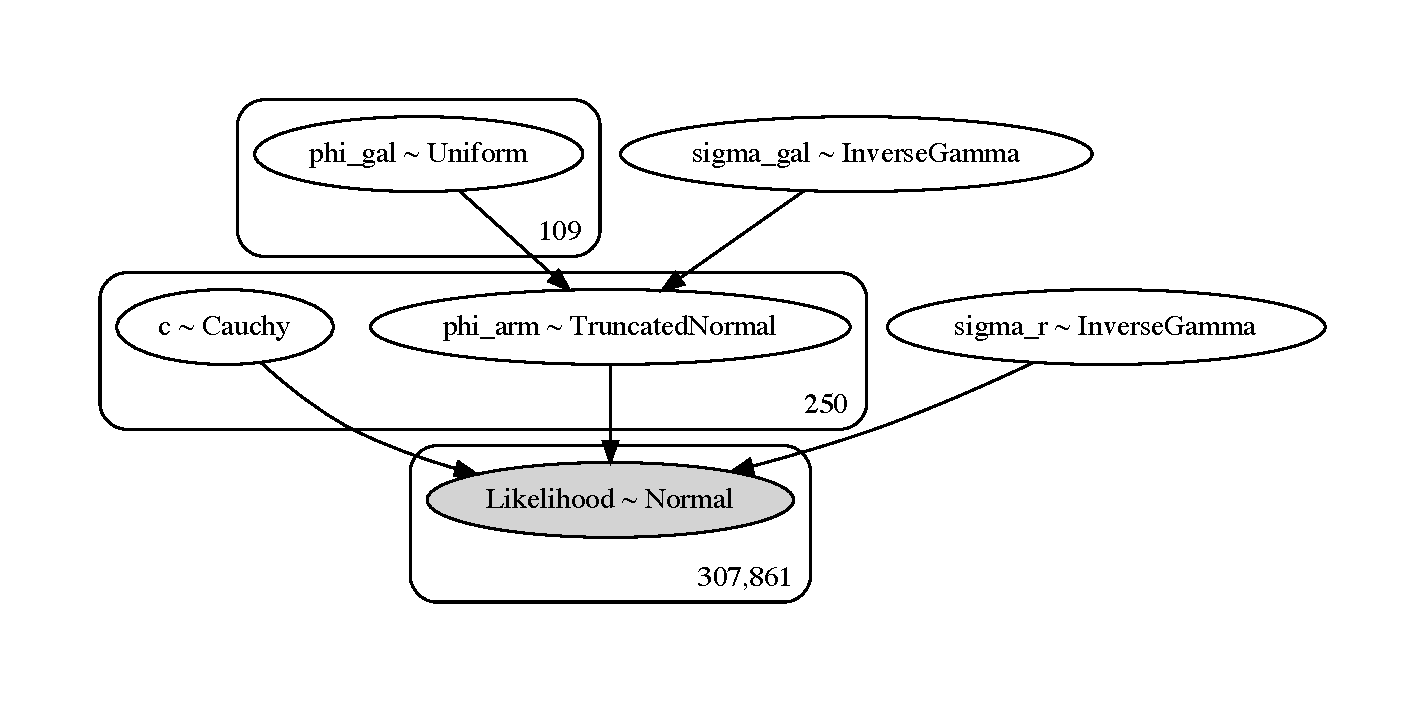
\includegraphics[width=8cm]{plots/plots_n109d1000t500/model.pdf}
  \caption{The model used for galaxy pitch angle measurement for the sample.}
  \label{fig:ad-cot-test}
\end{figure}

To perform inference, we make use of the No-U-Turn-Sampler (NUTS), implemented in PYMC3\footnote{\url{https://docs.pymc.io/}}, an open source probabilistic programming framework written in python. \comment{does PYMC3 have a citation?}
